\documentclass[11pt]{article}
% --- Encoding e font ---
\usepackage[utf8]{inputenc}
\usepackage[T1]{fontenc}
\usepackage{lmodern}

% --- Matematica ---
\usepackage{amsmath,amssymb,amsfonts,gensymb,amsthm}
\DeclareMathOperator*{\argmin}{arg\,min}
\DeclareMathOperator*{\argmax}{arg\,max}
\usepackage{centernot}
% --- Grafica, colori, float ---
\usepackage{graphicx}
\usepackage[dvipsnames]{xcolor}
\usepackage{float}
% --- Liste e ambienti ---
\usepackage{enumitem}
% --- Caption, numerazione figure ---
\usepackage{caption}
\usepackage{chngcntr}
% --- Caption, numerazione figure ---
\captionsetup{font=small, labelfont=bf, textfont=it}
% --- Indice/TOC personalizzazione (se ti serve) ---
\usepackage{tocloft}
% --- colorbox
\usepackage[most]{tcolorbox}
%--- spazio tra le riga
\usepackage{parskip}
\setlength{\parskip}{0.15cm}
% Elenchi compatti:
\setlist[itemize]{ topsep=2pt, itemsep=0pt, parsep=0pt}
\setlist[enumerate]{topsep=2pt, itemsep=0pt, parsep=0pt}

% Per il codice
\usepackage{listings}
% Definisci i colori esatti di VS Code (tema Light+)
\definecolor{vscodeblue}{RGB}{0,0,255}          % Keywords
\definecolor{vscodeorange}{RGB}{163,21,21}      % Strings
\definecolor{vscodegreen}{RGB}{0,128,0}         % Comments
\definecolor{vscodepurple}{RGB}{197,134,192}    % Control flow e import
\definecolor{vscodeyellow}{RGB}{121,94,38}      % Functions
\definecolor{vscodebg}{RGB}{255,255,255}        % Background
\definecolor{vscodeframe}{RGB}{200,200,200}     % Frame

% Configurazione Python stile VS Code
\lstdefinestyle{vscode}{
    language=Python,
    alsoletter={.},
    backgroundcolor=\color{vscodebg},
    commentstyle=\color{vscodegreen}\itshape,
    numberstyle=\tiny\color{gray},
    stringstyle=\color{vscodeorange},
    basicstyle=\ttfamily\small,
    breakatwhitespace=false,
    breaklines=true,
    captionpos=b,
    keepspaces=true,
    numbers=left,
    numbersep=8pt,
    showspaces=false,
    showstringspaces=false,
    showtabs=false,
    tabsize=4,
    frame=single,
    rulecolor=\color{vscodeframe},
    framesep=10pt,
    xleftmargin=15pt,
    framexleftmargin=15pt,
    % Resetta tutte le keyword e ridefiniscile
    morekeywords={},
    deletekeywords={for,if,while,else,elif,return,break,continue,try,except,finally,with,as,pass,raise,assert,import,from},
    % Keywords blu
    keywordstyle=\color{vscodeblue}\bfseries,
    morekeywords={def,class,lambda,and,or,not,is,in,del,global,nonlocal,yield,await,async,True,False,None,self},
    % Control flow VIOLA
    keywordstyle=[2]\color{vscodepurple}\bfseries,
    morekeywords=[2]{for,if,while,else,elif,return,break,continue,try,except,finally,with,as,pass,raise,assert,import,from},
    % Funzioni
    emph={sqrt,print,input,range,len,str,int,float,list,dict,set,tuple},
    emphstyle=\color{vscodeyellow}
}
\lstset{style=vscode}

%-- for definition (POI definisci defbox)
\newtcolorbox{defbox}[1]{
    colback=gray!10,
    colframe=gray!50,
    fonttitle=\bfseries,
    coltitle=black,
    title=\mbox{#1},  % Cambiato qui
    sharp corners,
    boxrule=0.5pt, breakable}
%-----
%-----
\usepackage{needspace}
%---- Notebox definition \begin{noteboxtitle}{title}
\newtcolorbox{noteboxtitle}[1]{
    colback=white,
    colframe=black!90,
    boxrule=0.8pt,
    arc=3mm,
    title=#1,
    fonttitle=\bfseries,
    left=5pt,
    right=5pt,
    top=5pt,
    bottom=5pt,
      breakable
}

% --- comment
\usepackage{comment}
% --- Margini ---
\usepackage[a4paper,
    top=2.5cm,
    bottom=2.5cm,
    left=2.5cm,
    right=2.5cm,
    bindingoffset=0.5cm
]{geometry}
% --- Titolo con immagine (opzionale) ---
\usepackage{titlepic} % solo se usi \titlepic
% --- Hyperref VA QUASI SEMPRE PER ULTIMO ---
\usepackage{hyperref}
\usepackage{adjustbox}
\usepackage{xltabular}
\usepackage{booktabs}
\raggedbottom


%---Per spezzare le tabelle
\usepackage{longtable}


% --- New structure for Example
\newtheoremstyle{smallexample}
  {3pt}% Space above
  {3pt}% Space below
  {\small}% Body font - testo dell'esempio piccolo
  {}% Indent amount
  {\small\bfseries}% Theorem head font - "Example 18.1" piccolo e grassetto
  {.}% Punctuation after theorem head
  {.5em}% Space after theorem head
  {}% Theorem head spec
\theoremstyle{smallexample}
\newtheorem{example}{Example}[section]
\usepackage[version=4]{mhchem}
\graphicspath{{Images/}}

 %% --- Definizione prima pagina 


%%___NEW COMMAND
\newcommand{\vs}{\vspace{0.2\baselineskip}}



%%%--- Librerie per grafici

\usepackage{tikz}
\usetikzlibrary{positioning, arrows.meta, shapes.geometric, calc}
\usepackage{tcolorbox}
\tcbuselibrary{breakable, skins}



\parindent 0px
\title{\Huge Data Mining and Machine Learning}
\author{\Large Gennaro Basile}
\date{\today}

\titlepic{
    \begin{center}
        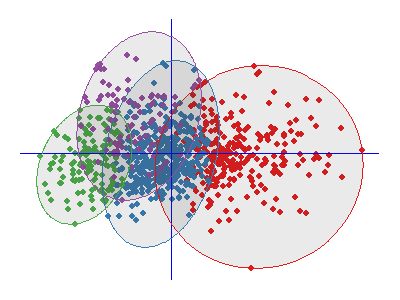
\includegraphics[scale=1]{0.png}
    \end{center}}



\begin{document}
\maketitle
\counterwithin{figure}{subsection}
\captionsetup[figure]{labelfont=bf}

\pagebreak

%% -- Sommario
\tableofcontents
\pagebreak


\section{Probability Model: The Foundation of Inference}

\subsection{Descriptive vs. Inferential Statistics}

In Data Science, we deal with two fundamentally different problems. It is crucial to distinguish them immediately.

\begin{defbox}{Descriptive Statistics (The Direct Problem)}
We observe the \textbf{entire population} (e.g., every single customer in a database).
\begin{itemize}
    \item \textbf{Goal:} Summarize the data exactly.
    \item \textbf{Result:} Certain facts (e.g., \textit{The exact average age is 35.2}).
    \item \textbf{Uncertainty:} Zero.
\end{itemize}
\end{defbox}

\begin{defbox}{Statistical Inference (The Indirect Problem)}
We only observe a small \textbf{sample} (e.g., 100 surveyed customers).
\begin{itemize}
    \item \textbf{Goal:} Infer the characteristics of the whole population based on the sample.
    \item \textbf{Result:} Estimates with uncertainty (e.g., \textit{The avg age is likely between 34 - 36}).
    \item \textbf{Tool:} We use Probability to measure that uncertainty.
\end{itemize}
\end{defbox}

\paragraph{Basic Definitions. }

To move from a sample to a population, we must formally define the entities involved and the goals of inference.
\begin{itemize}[label=$\cdot$]
    \item \textbf{Population}: the entire group under study to which conclusions are to be applied.
    \item \textbf{Sample}: a subset of the population that is actually observed and collected.
    \item \textbf{Statistical Inference}: The process of drawing conclusions about the population from data collected on a sample, using probability reasoning.
\end{itemize}

\subsubsection{The Two Main Tasks of Inference}
As a Data Scientist, you will mostly perform two tasks:
\begin{enumerate}
\item \textbf{Estimation:}  This involves estimating unknown population characteristics (parameters) based on sample statistics.
 \begin{itemize}
  \item \textbf{Point Estimation}: Assigning a single value to the population parameter (e.g., using the sample mean $\bar{x}$ to estimate the population mean $\mu$).
  \item \textbf{Interval Estimation}: Assigning an interval of plausible values (a confidence interval) to the parameter.
  \end{itemize}
    \item \textbf{Hypothesis Testing:} Deciding whether a claim (hypothesis) about a population parameter is acceptable or should be rejected, in probabilistic terms.(e.g., Did the new marketing campaign actually increase sales or was it just luck?).
\end{enumerate}

\vspace{0.2cm}
\begin{example}{\textbf{Parameter Estimation}}.

A Data Scientist wants to know the average age ($\mu$) of all customers of an e-commerce platform (Population). Since they cannot survey millions of users, they take a sample of $n=100$ customers.
\begin{itemize}
 \item \texttt{Step1 (Descriptive)}:
 \begin{itemize}
     \item Calculate the sample mean age. Suppose the sample mean is $\bar{x} = 35.2$ years.
 \end{itemize}
 \item \texttt{Step2 (Point Estimation)}:
 \begin{itemize}
     \item The point estimate for the population mean $\mu$ is $35.2$.
 \end{itemize}
 \item \texttt{Step3 (Interval Estimation)}:
 \begin{itemize}
     \item Based on sample var and size, they calculate a 95\% Confidence Interval for $\mu$, say $[34.0, 36.4]$. They infer that the true $\mu$ age of \textit{all} customers is likely between 34.0 and 36.4 y.o.
 \end{itemize} 
\end{itemize}
\end{example}

\subsubsection{The Importance of Unbiased Random Samples}

Since observations are made only on a sample, the fundamental questions are:
\begin{itemize}[label=-]
 \item How to extend sample conclusions to the population?
 \item What are the limits of validity and reliability of these conclusions?
\end{itemize}

The solution lies in using an \textbf{Unbiased Random Sample}:

\begin{itemize}
\item  A sample where the units are selected through a \textbf{random draw}, ensuring that the selection process is not influenced by the studied variable. This means every unit in the population has the same probability of being chosen.
\begin{itemize}
    \item This method is the best approach to \textbf{ensure representativeness and validity of inference}.
    \item If the survey is not random, inferential methods cannot be applied because the sample might not accurately reflect the population.
\end{itemize}
\end{itemize}

\subsection{Probability: The Measure of Uncertainty}

\subsubsection{Why Do We Need Probability?}

In the previous section, we learned that we often only have a \textbf{Sample}, but we want to know about the \textbf{Population}.
Because the sample is just a small piece of the whole, our conclusions are never 100\% certain.

\textbf{Probability} is the mathematical tool we use to measure that uncertainty. It allows us to say: \textit{I am 95\% confident that the average age is between 34 and 36,} rather than just guessing.

\subsubsection{The Three Definitions of Probability}

How do we actually define \textit{Chance}? There are three main schools of thought. As a Data Scientist, you will mostly use the \textbf{Classical} and \textbf{Frequentist} approaches, but \textbf{Subjectivist} is the basis of Bayesian Statistics.

\begin{enumerate}
    \item \textbf{Classical Probability (Gambling):}
    Used when all outcomes are equally likely (e.g., dice, cards).
    \[ P(E) = \frac{\text{Number of Favorable Outcomes}}{\text{Total Number of Possible Outcomes}} \]

\vs
    \item \textbf{Frequentist Probability (Simulation):}
    Used for repeatable experiments. Probability is the \textbf{relative frequency} of an event happening over a huge number of trials.
    \[ P(E) \approx \frac{\text{Count of Successes}}{\text{Count of Trials}} \quad (\text{as trials } \to \infty) \]

\vs
    \item \textbf{Subjectivist Probability (Belief):}
    Used when experiments cannot be repeated (e.g., \textit{Will humanity go to Mars by 2030?}). It measures a degree of personal belief or betting odds.
\end{enumerate}

\begin{example}{\textbf{Example: Tossing Coins}}

If you toss two coins, the Sample Space is $\{HH, HT, TH, TT\}$.
The event \texttt{Getting exactly one head} has 2 favorable outcomes ($HT, TH$).
\[ P(\text{One Head}) = \frac{2}{4} = 0.5 \]
\end{example}

\pagebreak
\subsection{Axioms and Fundamental Rules}

\subsubsection{Set Theory and Venn Diagrams}
We treat Probability mathematically using \textbf{Set Theory}. We visualize outcomes using \textbf{Venn Diagrams}.

\begin{itemize}[label=$\cdot$]
\item \textbf{Trial}: is a single execution of an experiment or process that results in an outcome (e.g.,The single roll of the die).

\vs
    \item \textbf{Sample Space ($S$):} the set of all possible outcomes of an experiment. The rectangle containing everything that can happen.

    \vs
    
    \item \textbf{Event ($A$):} a collection of outcomes, or a subset of the sample space S. A circle inside the rectangle representing a specific outcome. Events are combined using Boolean Logic Operators:  Union $\cup$, Intersection $\cap$,  Complement $\overline{A}$.
\end{itemize}


% IMMAGINE ORIGINALE MANTENUTA
\begin{figure}[H] 
    \centering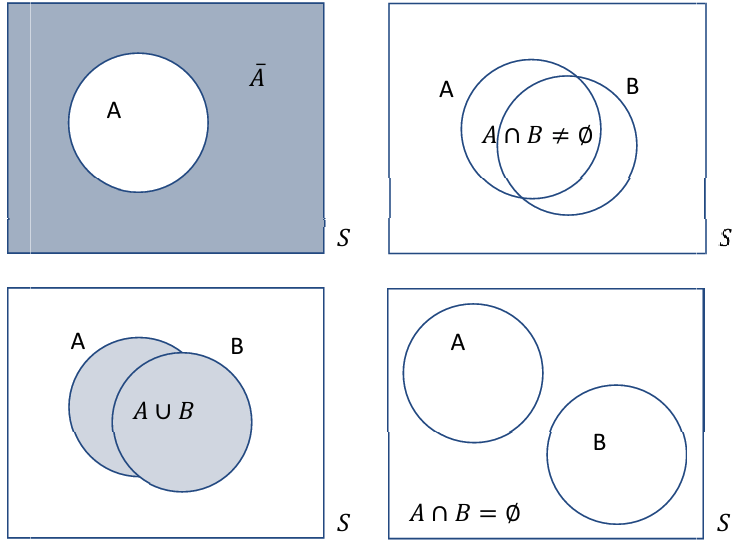
\includegraphics[scale=0.4]{103.Venn Diagram.jpeg}
    \caption{Venn Diagram}
    \captionsetup{font=footnotesize}
    \label{fig-Venn Diagram}
\end{figure}

\subsubsection{Kolmogorov's Three Axioms}
The \textbf{three fundamental axioms} define the mathematical properties that any probability measure $P$ must satisfy.

\begin{enumerate}
    \item \textbf{Positivity:} You cannot have a negative chance.
    \[ P(E) \ge 0 \]
    \item \textbf{Certainty:} The probability that \textit{something} in the sample space happens is 100\%.
    \[ P(S) = 1 \]
    \item \textbf{Additivity (for Disjoint Events):} If two events cannot happen at the same time (Mutually Exclusive, $A \cap B = \emptyset$), you just add their probabilities.
    \[ P(A \cup B) = P(A) + P(B) \]
\end{enumerate}

\subsubsection{Important Theorems derived from Axioms}

From those three simple rules, we derive the formulas you will use in practice.

\begin{itemize}
 \item \textbf{The Complement Rule}: The probability that an event $E$ does \textit{not} occur ($\overline{E}$) is one minus the probability that $E$ occurs. This implies that $0 \le P(E) \le 1$.
  \begin{equation}
      P(\overline{E}) = 1 - P(E)
  \end{equation}

    \item \textbf{The General Addition Law (Union):}
    If events $A$ and $B$ \textbf{can} overlap (happen together), we cannot just add them, or we would double-count the overlap. We must subtract the intersection.
    \[ P(A \text{ or } B) = P(A) + P(B) - P(A \text{ and } B) \]



 \item \textbf{Probability of the Empty Set ($\emptyset$)}: The probability of the impossible event is zero. This is derived from Axiom 3 (Additivity) and Axiom 2 (Unit Measure).
  \begin{equation}
      P(\emptyset) = 0
  \end{equation}
\end{itemize}


% IMMAGINE ORIGINALE MANTENUTA
\begin{figure}[H] 
    \centering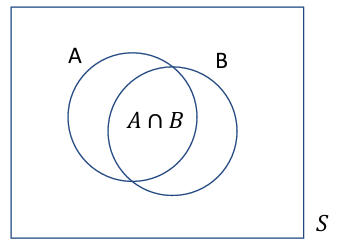
\includegraphics[scale=0.45]{104.Fundamental Theorems.jpeg}
    \caption{General Addition Law}
    \captionsetup{font=footnotesize}
    \label{fig-Fundamental Theorems}
\end{figure}

\begin{example}{\textbf{Example: Passing Exams}}

Let $P(Stat) = 0.60$ and $P(CS) = 0.50$.
If 35\% of students pass \textbf{both} ($P(Stat \cap CS) = 0.35$), what is the chance of passing \textbf{at least one}?
\[ P(Stat \cup CS) = 0.60 + 0.50 - 0.35 = 0.75 \]
\end{example}

\subsubsection{Extension: Three Events}
If you have three overlapping events ($A, B, C$), the logic is the same: Add the single circles, subtract the pairwise overlaps, and add back the center (because you subtracted it too many times).
\[ P(A \cup B \cup C) = P(A) + P(B) + P(C) - P(A \cap B) - P(A \cap C) - P(B \cap C) + P(A \cap B \cap C) \]

\subsection{Conditional Probability}

This is the most critical concept for understanding how Machine Learning models (like Naive Bayes) work. It answers: \textit{How do my chances change if I get new information?}

\subsubsection{Defining Conditional Probability}

\begin{defbox}{Conditional Probability}
The probability of event $B$ happening, \textbf{given that} we already know event $A$ has happened.
\begin{equation}
    P(B|A) = \frac{P(A \cap B)}{P(A)}
\end{equation}
\end{defbox}
We shrink the sample space. We no longer care about the whole world ($S$), only the world where $A$ is true.


\begin{defbox}{The Factorization Theorem (Total Probability)}
If we want to find the total probability of $B$, we sum up all the ways $B$ can happen (via $A$ or via $\bar{A}$):
\begin{equation}
    P(B) = P(A \cap B) + P(\bar{A} \cap B) =P(B|A)P(A) + P(B|\bar{A})P(\bar{A})
\end{equation}
\end{defbox}

\subsubsection{Stochastic Independence}
Two events are \textbf{Independent} if knowing $A$ gives us zero information about $B$.
\begin{equation}
    P(B|A) = P(B)
\end{equation}
If (and only if) this holds, we can just multiply probabilities: $P(A \cap B) = P(A) \cdot P(B)$.

\vspace{0.2cm}

\begin{example}{\textbf{Example 1: The Two-Way Table}}

Let's apply this to a real dataset.
$A$ = Female, $B$ = Wears Glasses.

% IMMAGINE ORIGINALE MANTENUTA
\begin{figure}[H] 
    \centering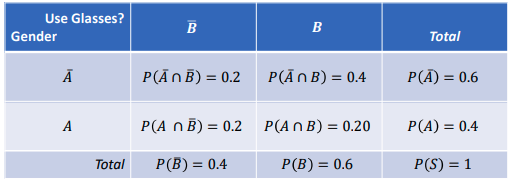
\includegraphics[scale=0.45]{136.Probability Two way table.jpeg}
    \caption{Probability Two way table}
    \captionsetup{font=footnotesize}
    \label{fig-Probability Two way table}
\end{figure}

\begin{itemize}
    \item \textbf{Question:} What is the probability a person wears glasses ($B$), \textit{given} they are Female ($A$)?
    \item \textbf{Calculation:} Look only at the \textit{Female} row.
    \[ P(B|A) = \frac{20 \text{ (Females with glasses)}}{40 \text{ (Total Females)}} = 0.5 \]
    \item \textbf{Check Independence:}
    $P(B) = 60/100 = 0.6$. Since $P(B|A) \neq P(B)$ ($0.5 \neq 0.6$), Gender and Glasses are \textbf{Dependent}.
\end{itemize}
\end{example}

\subsubsection{Bayes' Theorem}

This is the most important formula in Data Science. It tells us how to \textit{update our beliefs} when we see new evidence.

\begin{defbox}{Bayes' Theorem}
\begin{equation}
    P(A|E) = \frac{P(E|A) \cdot P(A)}{P(E)}
\end{equation}
\begin{itemize}
    \item $P(A)$: \textbf{Prior}. What we believed \textit{before} seeing data.
    \item $P(E|A)$: \textbf{Likelihood}. How probable is the evidence if our hypothesis is true?
    \item $P(A|E)$: \textbf{Posterior}. Our new belief \textit{after} seeing the evidence.
\end{itemize}
\end{defbox}

\subsubsection{Real World Application: Medical Diagnosis}
This is a classic interview question to test if you understand \textit{Base Rate Fallacy}.

\begin{example}{\textbf{The False Positive Paradox}}
\textbf{Scenario:}
\begin{itemize}
    \item A rare disease affects 1\% of people ($P(D) = 0.01$).
    \item The test is 95\% accurate ($P(+|D) = 0.95$).
    \item The test has a 10\% false positive rate ($P(+|\text{Health}) = 0.10$).
\end{itemize}
\textbf{Question:} You test positive. What is the probability you actually have the disease?

\textbf{The Calculation (Bayes):}
\[ P(D|+) = \frac{P(+|D) \cdot P(D)}{P(+)} \]

\begin{enumerate}
    \item \textbf{Numerator (True Positive path):} $0.95 \times 0.01 = 0.0095$
    \item \textbf{Denominator (Total Positives):}
    True Positives + False Positives
    \[ (0.95 \times 0.01) + (0.10 \times 0.99) = 0.0095 + 0.099 = 0.1085 \]
    \item \textbf{Result:}
    \[ \frac{0.0095}{0.1085} \approx \textbf{8.76\%} \]
\end{enumerate}

\textbf{Conclusion:} Even with a positive test, you are likely healthy! Why? Because the disease is so rare ($1\%$) that the false alarms ($10\%$ of the $99\%$ healthy people) drown out the real cases.
\end{example}



\subsection{Combinatorial Calculus and Discrete Random Variables}

\subsubsection{Combinatorial Calculus}

Before calculating probabilities, we often need to count how many ways something can happen. This is \textbf{Combinatorics}.

\begin{defbox}{Ordered Sequences (Does Order Matter? YES)}
\textbf{1. With Replacement:}
You have $n$ options, and you choose $k$ times. After each choice, you put the item back.
\begin{equation}
n^k
\end{equation}
\begin{itemize}
    \item \textit{Example:} A 4-digit PIN code ($10^4 = 10,000$ codes).
\end{itemize}

\vs
\textbf{2. Without Replacement (Permutations):}
You have $n$ options, choose $k$. Once picked, an item is gone
\begin{equation}
D_{n,k} = \frac{n!}{(n-k)!}
\end{equation}
\begin{itemize}
    \item \textit{Example:} A race with 8 runners. Who gets Gold, Silver, and Bronze ($k=3$)?

\end{itemize}
\end{defbox}

\begin{defbox}{Unordered Sequences (Does Order Matter? NO)}
\textbf{Combinations (The Binomial Coefficient):}
You choose $k$ items from $n$, and the order does \textbf{not} matter.
    \begin{equation}
        C_{n,k} = \binom{n}{k} = \frac{n!}{k!(n-k)!}
    \end{equation}
\begin{itemize}
    \item \textit{Example:} Choosing a team of 3 Data Scientists from a department of 8.
\end{itemize}
\end{defbox}

This is the most critical formula for Data Science (used in sampling).

\subsubsection{Discrete Random Variables}

A \textbf{Random Variable} ($X$) is just a function that translates a \textit{real world outcome} into a number. It is \textbf{Discrete} because can only take specific integer values (e.g., number of sales, number of clicks).


\pagebreak
\begin{example}{\textbf{Discrete Random Variable}}

  Imagine an experiment, like flipping a coin three times. The raw outcomes (elementary events) are: {HHH, HHT, HTH, THH, HTT, THT, TTH, TTT}.
  
  \vs
  The Discrete Random Variable ($X$) is defined as the "Number of Heads" in the three flips: 3, 2, 2, ...  
\end{example}

         \begin{figure}[H] 
        \centering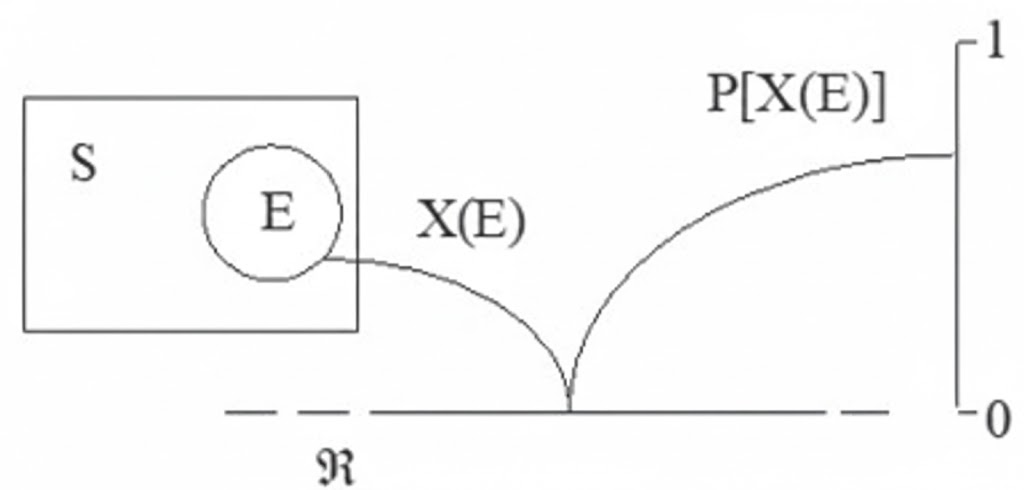
\includegraphics[scale=0.2]{106.Discrete variable.jpeg}
        \caption{Discrete Random variable}
        \captionsetup{font=footnotesize}
        \label{fig-Discrete Random variable}
    \end{figure}


\begin{defbox}{Key Metrics: Mean and Variance}
\textbf{1. Expected Value (mean):}
If you repeated the experiment infinitely, what would be the average?
\begin{equation}
    E(X) = \mu = \sum x_i \cdot p_i
\end{equation}

\textbf{2. Variance:}
How far are the values typically from the mean?
\begin{equation}
    \text{Var}(X) = E[(X - \mu)^2]
\end{equation}
\end{defbox}


\subsubsection{Discrete Probability Models}

In the previous section, we learned what a Random Variable is (a way to map outcomes to numbers). Now we'll explore several important \textbf{probability distributions} that model common real-world scenarios.

Think of these as  \textit{patterns} that describe how data behaves in the real world. Once you recognize the pattern (e.g., \textit{counting successes}), you can just pick the right tool (e.g., \textit{Binomial}) and use its ready-made formulas.

\vspace{0.3cm}
\textbf{1. The Basic Building Blocks}


\vspace{0.05cm}

\begin{defbox}{Uniform Distribution $U(k)$}
\textbf{Scenario:} \textit{Everything is equally likely.}
\begin{itemize}
    \item \textbf{Example:} Rolling a fair die.
    \item \textbf{Probability:} $P(X=x) = \frac{1}{k}$
    \item \textbf{Mean:} The exact middle value.
\end{itemize}
\end{defbox}

\vs
\begin{defbox}{Bernoulli Distribution $B(1, \pi)$}
\textbf{Scenario:} \textit{The Atom of Probability.} A single trial with only two outcomes: Success (1) or Failure (0).
\begin{itemize}
    \item \textbf{Example:} A user clicks an ad (Yes/No).
    \item \textbf{Parameter $\pi$:} The probability of success.
    \item \textbf{Mean:} $\pi$.
    \item \textbf{Variance:} $\pi(1-\pi)$ (Variance is highest when $\pi=0.5$: maximum uncertainty).
\end{itemize}
\end{defbox}

\vs
\textbf{2. Counting Successes (The \textit{Binomial} Family)}

These distributions answer the question: \textit{How many successes did I get?}

\vs

\begin{defbox}{Binomial Distribution $B(n, \pi)$}
\textbf{Scenario:} You repeat a Bernoulli trial $n$ times independently.
\begin{itemize}
    \item \textbf{Example:} 100 users visit your site ($n=100$), and each has a 5\% chance of buying ($\pi=0.05$). How many sales ($X$) do I get?
    \item \textbf{Formula:} Uses the combination $\binom{n}{x}$.
    \item \textbf{Mean:} $n\pi$ (Expected sales = $100 \times 0.05 = 5$).
\end{itemize}
\end{defbox}

\vs

\begin{defbox}{Hypergeometric Distribution $H(N, n, m)$}
\textbf{Scenario:} Same as Binomial, but \textbf{Sampling Without Replacement}.
\begin{itemize}
    \item \textbf{Example:} You have a deck of 52 cards ($N$), with 4 Aces ($m$). You draw 5 cards ($n$). How many are Aces?
    \item \textbf{Key Difference:} The trials are \textbf{dependent}. If you draw an Ace first, it's harder to draw another one.
    \item \textbf{Usage:} Important for Quality Control (sampling from small batches).
\end{itemize}
\end{defbox}

\vspace{0.3cm}

\textbf{3. Waiting Time (The \textit{Geometric} Family)}

These distributions answer the question: \textit{How long do I have to wait?}

\begin{defbox}{Geometric Distribution $G(\pi)$}
\textbf{Scenario:} How many trials until the \textbf{first} success?
\begin{itemize}
    \item \textbf{Example:} How many job interviews until I get an offer? (assuming 20\% success rate).
    \item \textbf{Mean:} $1/\pi$ (If success rate is 20\%, expect to wait 5 interviews).
    \item \textbf{Property:} \textit{Memoryless}. If you failed 10 times, your probability on the 11th try is exactly the same.
\end{itemize}
\end{defbox}

\vs
\begin{defbox}{Negative Binomial $NB(k, \pi)$}
\textbf{Scenario:} How many trials until the \textbf{$k$-th} success?
\begin{itemize}
    \item \textbf{Example:} How many cold calls to make 5 sales?
    \item It is essentially the sum of $k$ independent Geometric variables.
\end{itemize}
\end{defbox}

\vspace{0.3cm}
\textbf{4. Rate of Events (Poisson)}

\vs
\begin{defbox}{Poisson Distribution $P(\lambda)$}
\textbf{Scenario:} Modeling rare events over a fixed time or space.
\begin{itemize}
    \item \textbf{Example:} Number of server crashes per month. Number of customers arriving per hour.
    \item \textbf{Parameter $\lambda$:} The average rate of occurrence.
    \item \textbf{Unique Property:} Mean = Variance = $\lambda$.
    \item \textbf{Usage:} Crucial for queuing theory and reliability engineering.
\end{itemize}
\end{defbox}

% IMMAGINE ORIGINALE MANTENUTA
\begin{figure}[H] 
    \centering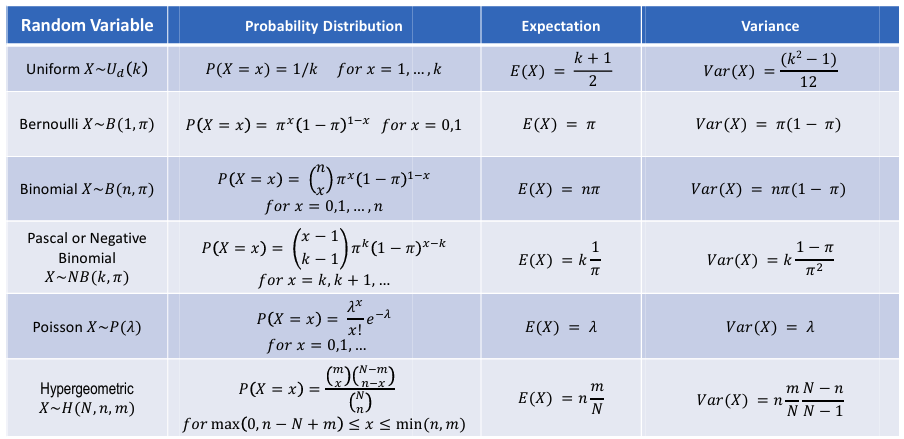
\includegraphics[scale=0.5]{107.Discrete probabilty model tabel.jpeg}
    \caption{Discrete probabilty model tabel}
    \captionsetup{font=footnotesize}
    \label{fig-Discrete probabilty model tabel}
\end{figure}
\end{document}

